
\chapter{Química Cuantitativa}

\section{Introducción}
Se define la Química (del egipcio \emph{Keme}, “tierra”) como la ciencia que estudia la estructura, propiedades, composición y transformación de la materia. La química moderna se desarrolló a partir de la alquimia, una práctica protocientífica de carácter filosófico, que combinaba elementos de la química, la metalurgia, la física, la medicina, la biología, entre otras ciencias y artes. Esta fase termina al ocurrir la llamada,Revolución de la Química, basada en la Ley de conservación de la Masa y la teoría de la combustión por oxígeno postuladas por el científico francés, Antoine L. Lavoisier. \\
La Química a veces es definida como La Ciencia Central a causa de su rol de conexión y articulación entre las ciencias físicas, de las cuales forma parte, junto con las ciencias de la vida, y algunas ciencias aplicadas como la medicina o la ingeniería.

\section{Leyes Ponerales}

Las leyes ponderales de la Química son un conjunto de leyes de carácter empírico desarrolladas entre 1789 y 1803 por los primeros químicos que trataban de encontrar relaciones entre las masas de los compuestos químicos que intervenían en una reacción química. Posteriormente fueron generalizadas y superadas con la aparición de la teoría atómica y el concepto de mol.

\subsection{Ley de la Conservación de la Masa (Ley de Lavoisier)}

\textbf{Antonie-Laurent de Lavoisier (1743-1794)}, fue el primer químico que realizó cuidadosamente mediciones con la balanza, obteniendo una explicación correcta de las reacciones en las que metales como mercurio o cobre eran calentados en presencia de aire. En 1789, Lavoisier generalizó sus resultados a todas las reacciones químicas enunciando la llamada \emph{Ley de conservación de la masa}:\\
\begin{law}[Ley de Lavoisier]
En una reacción química, la masa total de las substancias que reaccionan (reactivos) es igual a la masa total de las substancias formadas (productos)
\begin{align}
\sum_{i = 1}^{N}(m_i)_{reactivos} = \sum_{i = 1}^{N}(m_i)_{productos}
\end{align}
\end{law}
\begin{figure}[h!]
	\centering
	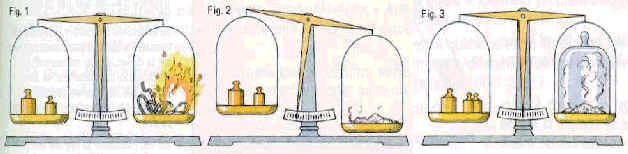
\includegraphics{lavoisier}
\end{figure}

\subsection{Ley de las Proporciones Definidas (Ley de Proust)}

Si en condiciones cuidadosamente controladas, hacemos reaccionar por ejemplo, 10 g de cloro con 10 g de sodio, podrá probarse que los 10 g de cloro no reaccionan con todo el sodio, sino solo con una porción de él (6,484 g exactamente) quedándose el exceso sin reaccionar. Según la experiencia, el cloro y el sodio han reaccionado en la proporción en peso:\\

\begin{center}
	$\frac{m_{Na}}{m_{Cl}}=\frac{6,484}{10}$
\end{center}

\begin{law}[Ley de Proust]
	Cuando dos o más elementos se combinan para formar un determinado compuesto lo hacen en una relación en peso constante independientemente del proceso seguido para formarlo.
\end{law}
\\
Esta ley fue enunciada por \emph{Louis Proust} en 1799, y atacada por \emph{C. L. Berthollet}, quién creía que la composición de un compuesto variaba según el método por el que se había preparado.\\

Modernamente se conocen compuestos sólidos que no cumplen la ley de las proporciones definidas (óxidos y sulfuras de elementos de transición), y se les llama compuestos no estequiométricos o \emph{Compuestos Berthóllidos}.\\

Podemos decir por tanto que:

\begin{center}
		$\frac{m_{Na}}{m_{Cl}}=\frac{6,484}{10}=\frac{12,968}{20}=\frac{4,934}{7,61}=cte$
\end{center}

Cada muestra de sal común descompuesta nos arrojará invariablemente un 39,34 \% de sodio y un 60,66 \% de cloro (relación 6,484/10)

\subsection{Ley de las Proporciones Definidas (Ley de Dalton)}

La ley anterior no excluye la posibilidad de que dos sustancias puedan formar compuestos diferentes si varían las condiciones experimentales. De hecho, esto es lo que sucede, por ejemplo, con el oxígeno y el hierro o el cobre o el carbono, que dependiendo de las condiciones de la experiencia se originan óxidos diferentes. Para cada proceso individual, se cumple, por supuesto la ley de Proust, sin embargo, cabe hablar de otra más general que incluye estos casos. Veamos un ejemplo:\\

Al hacer reaccionar un gramo de oxígeno con cobre, la cantidad de éste consumida es exactamente 3,971 g:

\begin{center}
	$Oxígeno (1 gr) + Cobre  (3,971 gr) \rightarrow Óxido de Cobre
	$ 
\end{center}

Pero en condiciones experimentales diferentes, un gramo de oxígeno puede reaccionar con 7,942 g de cobre para dar lugar a otro compuesto diferente:

\begin{center}
	$Oxígeno (1 gr) + Cobre (7,942 gr) \rightarrow Óxido de Cobre’ $
\end{center}

Si dividimos los gramos de cobre que en ambos casos se combinaron con la misma cantidad (un gramo) de oxígeno, veremos que resulta una relación muy sencilla:

\begin{center}
	$\frac{3,971}{7,942}=\frac{1}{2}$
\end{center}

Lo anterior es un ejemplo de la Ley de las Proporciones Múltiples enunciada en 1803 por \emph{J. Dalton}:\\

\begin{law}[Ley de Dalton de las Proporciones Múltiple]
	Las cantidades de un mismo elemento que se combinan con una cantidad fija de otro para formar varios compuestos están en la relación de los números enteros sencillos
\end{law}

\subsection{Ley de las Prporciones Equivalentes (Ley de Richter)}

Fue enunciada por primera vez por \emph{J.B. Richter} en 1792. Es de importancia para la historia de la química y el desarrollo del concepto de mol y de fórmula química más que para la química actual. Esta ley permite establecer el peso equivalente o peso-equivalente-gramo, que es la cantidad de un elemento o compuesto que reaccionará con una cantidad fija de una sustancia de referencia.\\

\begin{law}[Ley de Richter]
	
	Las masas de dos elementos diferentes que se combinan con una misma cantidad de un tercer elemento, guardan la misma relación que las masas de aquellos elementos cuando se combinan entre sí.
\end{law}

\section{Leyes Volumétricas}

Son un conjunto de leyes de naturaleza empírica que relaciona los volúmenes de gases que intervienen en una reacción química.

\subsection{Ley de los Volúmenes de Combinación de Gay-Lussac)}

\emph{Joseph Louis Gay-Lussac} (1778-1850) estudió las reacciones en las que intervenían gases, realizando sus estudios en reacciones a Presión y Temperatura constantes. Tras estudiar distintos tipos de reacciones químicas (siempre en fase gaseosa) llegó a la conclusión que ocurría algo análogo a la la Ley de Proust cuando se medían los distintos volumenes de las sustancias intervinientes en la reacción.\\

\begin{figure}[h!]
	\centering
	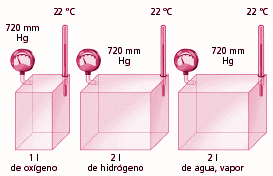
\includegraphics {vcgaylussac}
\end{figure}

\begin{law}[Ley de los Volúmenes de Combinación de Gay-Lussac]
	Los volúmenes de las sustancias gaseosas que intervienen en una reacción química, medidos en las mismas condiciones de presión y temperatura, están en relación de números enteros sencillos.
\end{law}